%%%%%%%%%%%%%%%%%%%%%%%%%%%%%%%%%%%%%%%%%
% Short Sectioned Assignment LaTeX Template Version 1.0 (5/5/12)
% This template has been downloaded from: http://www.LaTeXTemplates.com
% Original author:  Frits Wenneker (http://www.howtotex.com)
% License: CC BY-NC-SA 3.0 (http://creativecommons.org/licenses/by-nc-sa/3.0/)
%%%%%%%%%%%%%%%%%%%%%%%%%%%%%%%%%%%%%%%%%

%----------------------------------------------------------------------------------------
%	PACKAGES AND OTHER DOCUMENT CONFIGURATIONS
%----------------------------------------------------------------------------------------

\documentclass[paper=a4, fontsize=11pt]{scrartcl} % A4 paper and 11pt font size

% ---- Entrada y salida de texto -----

\usepackage[T1]{fontenc} % Use 8-bit encoding that has 256 glyphs
\usepackage[utf8]{inputenc}

% ---- Idioma --------

\usepackage[spanish, es-tabla]{babel} % Selecciona el español para palabras introducidas automáticamente, p.ej. "septiembre" en la fecha y especifica que se use la palabra Tabla en vez de Cuadro

% ---- Otros paquetes ----

\usepackage{amsmath,amsfonts,amsthm} % Math packages
\usepackage{graphics,graphicx, floatrow} %para incluir imágenes y notas en las imágenes
\usepackage{graphics,graphicx, float} %para incluir imágenes y colocarlas
\usepackage{hyperref} % url in references
\usepackage{textcomp}
\usepackage{listings}
\usepackage{titlesec}

% Para hacer tablas comlejas
\usepackage{multirow}
\usepackage{threeparttable}

\usepackage{fancyhdr} % Custom headers and footers
\pagestyle{fancyplain} % Makes all pages in the document conform to the custom headers and footers
\fancyhead{} % No page header - if you want one, create it in the same way as the footers below
\fancyfoot[L]{} % Empty left footer
\fancyfoot[C]{} % Empty center footer
\fancyfoot[R]{\thepage} % Page numbering for right footer
\renewcommand{\headrulewidth}{0pt} % Remove header underlines
\renewcommand{\footrulewidth}{0pt} % Remove footer underlines
\setlength{\headheight}{13.6pt} % Customize the height of the header

\numberwithin{equation}{section} % Number equations within sections (i.e. 1.1, 1.2, 2.1, 2.2 instead of 1, 2, 3, 4)
\numberwithin{figure}{section} % Number figures within sections (i.e. 1.1, 1.2, 2.1, 2.2 instead of 1, 2, 3, 4)
\numberwithin{table}{section} % Number tables within sections (i.e. 1.1, 1.2, 2.1, 2.2 instead of 1, 2, 3, 4)

\setlength\parindent{0pt} % Removes all indentation from paragraphs - comment this line for an assignment with lots of text

\newcommand{\horrule}[1]{\rule{\linewidth}{#1}} % Create horizontal rule command with 1 argument of height

\usepackage{textcomp}

%----------------------------------------------------------------------------------------
%	DATOS
%----------------------------------------------------------------------------------------

\newcommand{\myName}{Francisco Javier Bolívar Lupiáñez}
\newcommand{\myDegree}{Grado en Ingeniería Informática}
\newcommand{\myFaculty}{E. T. S. de Ingenierías Informática y de Telecomunicación}
\newcommand{\myDepartment}{Lenguajes y Sistemas de Información}
\newcommand{\myUniversity}{\protect{Universidad de Granada}}
\newcommand{\myLocation}{Granada}
\newcommand{\myTime}{\today}
\newcommand{\myTitle}{Trabajo propuesto}
\newcommand{\mySubtitle}{Cómo afecta el tamaño del problema y el número de procesadores a la eficiencia de un algoritmo paralelo}
\newcommand{\mySubject}{Programación Paralela}
\newcommand{\myYear}{2015-2016}

%----------------------------------------------------------------------------------------
%	PORTADA
%----------------------------------------------------------------------------------------


\title{	
	\normalfont \normalsize 
	\textsc{{\bf \mySubject \space (\myYear)} \\ \myDepartment} \\[20pt] % Your university, school and/or department name(s)
	\textsc{\myDegree \\[10pt] \myFaculty \\ \myUniversity} \\[25pt]
	\horrule{0.5pt} \\[0.4cm] % Thin top horizontal rule
	\huge \myTitle: \mySubtitle \\ % The assignment title
	\horrule{2pt} \\[0.5cm] % Thick bottom horizontal rule
	\normalfont \normalsize
}

\author{\myName} % Nombre y apellidos

\date{\myTime} % Incluye la fecha actual
%----------------------------------------------------------------------------------------
%	INDICE
%----------------------------------------------------------------------------------------

\begin{document}
	
\setcounter{page}{0}

\maketitle % Muestra el Título
\thispagestyle{empty}

\newpage %inserta un salto de página

\tableofcontents % para generar el índice de contenidos

\listoffigures

\newpage

%----------------------------------------------------------------------------------------
%	DOCUMENTO
%----------------------------------------------------------------------------------------

\section{Planteamiento del problema}

Se pretende demostrar por qué la eficiencia (E) tiende a aumentar al aumentar el tamaño del problema (N) y a disminuir al aumentar el número de procesadores (P).

\section{Demostración}

\subsection{Modelo matemático}

Para demostrarlo se va a plantear un ejemplo y se utilizará el del \textbf{algoritmo del patrón de once puntos} visto en clase con una pequeña modificación: \textbf{la matriz tiene el mismo tamaño en todas las direcciones} (NxNxN). Este algoritmo realiza operaciones sobre una matriz 3D y para computar cada punto hace falta conocer el valor de sus vecinos de arriba y abajo, dos a la izquierda, dos a la derecha, dos hacia delante y dos hacia atrás, además del propio punto (Figura \ref{fig:oncePuntos}).

\begin{figure}[H]
	\centering
	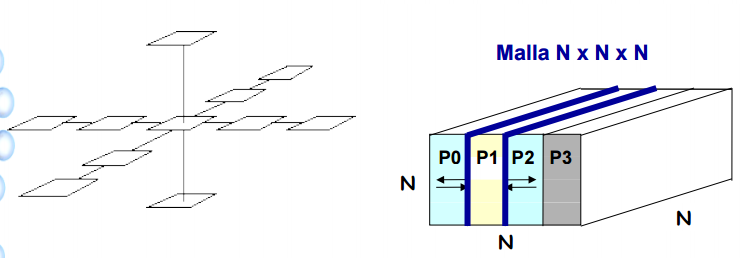
\includegraphics[width=10cm]{imagenes/oncePuntos}
	\caption{Patrón de once puntos, tamaño de la malla y reparto de ésta entre los procesos}
	\label{fig:oncePuntos}
\end{figure}

El tiempo de un algoritmo secuencial sería ($T_{1}$):
\begin{equation}
	T_{1} = t_{c}N^{3}
\end{equation}

Cuando se paraleliza, se reparten bloques de la matriz como se muestra en la Figura \ref{fig:oncePuntos}, por tanto cada proceso necesitará intercambiar $2N^{2}$ puntos con dos vecinos. Lo que hace que el tiempo de comunicación ($T_{comm}$) sea:
\begin{equation}
	T_{comm} = 2(t_{s} + t_{w}2N^{2})
\end{equation}

Y el tiempo de computación ($T_{comp}$):
\begin{equation}
	T_{comp} = \dfrac{t_{c}N^{3}}{P} 
\end{equation}

Por tanto el tiempo del algoritmo paralelizado ($T_{p}$) sería:
\begin{equation}
	T_{p} = T_{comp} + T_{comm} = \dfrac{t_{c}N^{3}}{P} + 2t_{s} + t_{w}4N^{2}
\end{equation}

La ganancia de velocidad (S) se calcula como la división del algoritmo secuencial ($T_{1}$) entre el paralelo ($T_{p}$):
\begin{equation}
	S = \dfrac{T_{1}}{T_{p}} = \dfrac{t_{c}N^{3}}{\dfrac{t_{c}N^{3}}{P} + 2t_{s} + t_{w}4N^{2}}
\end{equation}

Y la eficiencia (E), finalmente, se calcularía como la división entre la ganancia de velocidad (S) entre el número de procesadores (P):

\begin{equation}
	E = \dfrac{S}{P} = \dfrac{t_{c}N^{3}}{P( \dfrac{t_{c}N^{3}}{P} + 2t_{s} + t_{w}4N^{2})} = \dfrac{N^{3}t_{c}}{N^{3}t_{c} + 2Pt_{s} + 4PN^{2}t_{w}}
\end{equation}

En esta función resultante contamos con cinco variables:
\begin{itemize}
	\item $t_{c}$: tiempo de computación por punto.
	\item $t_{s}$: tiempo de inicialización de comunicación.
	\item $t_{w}$: tiempo de comunicación por palabra.
	\item N: tamaño de la matriz.
	\item P: número de procesadores.
\end{itemize}

Las tres primeras no varían, y se va a suponer que $t_{c}$ = 1 y $t_{s}$ = $t_{w}$ = 0.5. Por lo que vamos a utilizar la siguiente función para obtener los tiempos variando N y P:

\begin{equation}
	f(N,P) = \dfrac{N^{3}}{N^{3} + P + 2PN^{2}}
\end{equation}

\subsection{Mediciones y resultados}

Se toman tiempos con 10, 40, 70 y 100 procesadores y con tamaños de 100, 400, 700 y 1000. Obteniendo los siguientes resultados:

\begin{figure}[H]
	\centering
	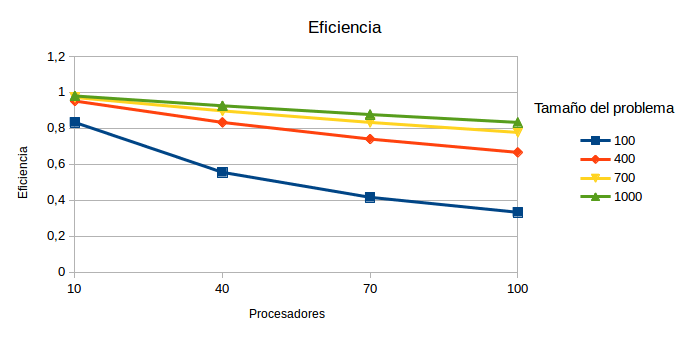
\includegraphics[width=14cm]{imagenes/grafico1}
	\caption{La eficiencia disminuye conforme se aumenta el número de procesadores}
	\label{fig:grafico1}
\end{figure}


\begin{figure}[H]
	\centering
	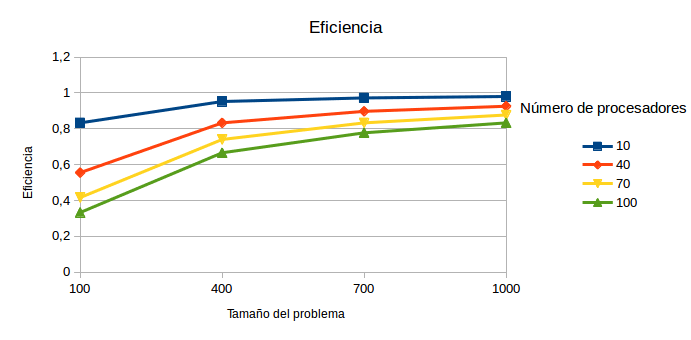
\includegraphics[width=14cm]{imagenes/grafico2}
	\caption{La eficiencia aumenta conforme se aumenta el tamaño del problema}
	\label{fig:grafico2}
\end{figure}

\end{document}